\section{Интуиция и формализация}

Итак, мы подошли к самомму важному что нам нужно из теории вероятности в алгоритмах. Чаще всего нас интересует вопрос: <<вот если мы поместим наш алгоритм в реальный мир, где вход случаен, то за сколько примерно это все будет работать?>>. Это есть некоторая другая призма взгляда на время работы, ежели когда мы смотрим <<худший случай>> работы. Ведь если худший случай, например, всего 1 и мы работаем в нем за $\O\left(n^2\right)$ и мы объективно понимаем, что он маловероятен, а во всех остальных случаях мы работаем условно за $\O(1)$, то логично сказать, что <<мы работаем за плюс-минус $\O(1)$ на случайных данных>>.

Давайте подведём под это формализацию. Будем считать, что мы работаем на некотором вероятностном пространстве $(\Omega, \mathcal{F}, \Pr)$ и на нем задали \textit{дискретную} случайную величину $\xi: \Omega \to \R$ (случай абсолютно непрерывных в курсе не рассматривается).

Рассмотрим частный пример -- бросание монеты. Для начала считаем, что монетка честная и что орёл, что решка выпадают равноверноятно. Если выпал орёл, то считаем, что $\xi$ принимает 0, а решка -- 1.
Коль скоро выпадение 1 и 0 равновероятно, то логично сказать, что всегда нужно ожидать <<что-то примерно между 0 и 1 по середине>>, т.е. $\frac{1}{2}$ (это назовем математическим ожиданием и обозначать будем $\E \xi$).

\begin{center}
    \begin{tikzpicture}[x=2.2cm, y=1cm]
        \draw[->, thick] (-0.6,0) -- (2.2,0) node[right] {$\R$};
        \foreach \x in {0,1} {
            \draw[thick] (\x,0.12) -- (\x,-0.12);
        }
        \fill (0,0) circle[radius=4.5pt];
        \fill (1,0) circle[radius=4.5pt];
        \fill[blue] (0.5,0) circle[radius=3.5pt];
        \node[below=8pt] at (0,0) {$0$};
        \node[below=8pt] at (1,0) {$1$};
        \node[above=6pt] at (0,0) {$\tfrac{1}{2}$};
        \node[above=6pt] at (1,0) {$\tfrac{1}{2}$};
        \node[blue, below=8pt] at (0.5,0) {$\E\xi$};
    \end{tikzpicture}
\end{center}

А давайте теперь возьмем и модифицируем монетку так, чтобы решка выпадала с вероятностью $\frac{2}{3}$, а орёл -- $\frac{1}{3}$.

\begin{center}
    \begin{tikzpicture}[x=2.2cm, y=1cm]
        \draw[->, thick] (-0.6,0) -- (2.2,0) node[right] {$\R$};
        \foreach \x in {0,1} {
            \draw[thick] (\x,0.12) -- (\x,-0.12);
        }
        \fill (0,0) circle[radius=3pt];
        \fill (1,0) circle[radius=6pt];
        \fill[blue] (2/3,0) circle[radius=3.5pt];
        \node[below=8pt] at (0,0) {$0$};
        \node[below=8pt] at (1,0) {$1$};
        \node[above=6pt] at (0,0) {$\tfrac{1}{3}$};
        \node[above=6pt] at (1,0) {$\tfrac{2}{3}$};
        \node[blue, below=8pt] at (2/3,0) {$\E\xi$};
    \end{tikzpicture}
\end{center}

Теперь кажется, что все таки коль скоро решка выпадает почаще, то и ожидать значение стоит более близкое к единице. Увеличившаяся вероятность выпадение решки, как бы сместила <<центр масс>>. Но уже чему тут равно математическое ожидание сложно без определения.

Итак, что мы хотим базово от математического ожидания:
\begin{enumerate}
    \item Его значения должны быть <<зажаты>> между значениями случайной величины (если случайная величина принимает значения 0 или 1, глупо ожидать, что она примет примерно значение 2).
    \item Должно отражать вероятностное распределение значений. То есть значение математического ожидания как-будто должно быть более близко по значению к тем числам, которые более вероятно встречаются, ежели наоборот, ведь они скорее всего и выпадут и их логично ожидать.
\end{enumerate}

Под такую модель подходит идеально взвешенная сумма значений случайной величины, где за веса мы будем брать вероятность. Таким образом если вероятность выпадения решки больше, то в сумме она будет больше доминировать и математическое ожидание сместится ближе к 1.

\Def \textit{Математическим ожидание} (или сокращенно \textit{матожидание}) случайной величины $\xi: \Omega \to \R$ будем назвать следующую величину:
\begin{equation*}
    \E \xi = \sum\limits_{\xi_0 \in \Img \xi} \xi_0 \Pr[\xi = \xi_0]
\end{equation*}

То есть теперь мы можем формально посчитать матожидание для монетки. Для честной оно выглядит следующим образом:
\begin{equation*}
    \E \xi = \frac{1}{2} \cdot 1 + \frac{1}{2} \cdot 0 = \frac{1}{2}
\end{equation*}
Получилось как мы и прогнозировали. А вот для второго случая теперь давайте посчитаем:
\begin{equation*}
    \E \xi = \frac{2}{3} \cdot 1 + \frac{1}{3} \cdot 0 = \frac{2}{3}
\end{equation*}
То есть как мы и хотели, матожидание сдвинулось ближе к единице.

\Exe Пусть $\xi$ и $\eta$ -- случайные величины. Покажите, что $\forall \alpha, \beta \in \R \hookrightarrow \E[\alpha \xi + \beta \eta] = \alpha \E \xi + \beta \E \eta$.

\Exe Пусть $\xi \equiv c$ -- константа. Пожажите, что $\E \xi = c$.

\Exe Пусть $\xi$ и $\eta$ -- случайные величины. Верно ли, что из $\E \xi = \E \eta$ следует $\xi \overset{\Omega}{=} \eta$ (совпадают на всем $\Omega$)?

\Exe Пусть $\xi$ -- равномерно распределенная величина. Покажите, что матожидание $\xi$ есть просто среднее арифметическое ее значений.

Также существует еще одна характеристика связанная с математическим ожиданием. Она возникает, когда мы хотим ответить на вопрос: <<а на сколько величина $\xi$ отличается от своего матождания в среднем?>>. Эта величина назвается \textit{дисперсия}.

\Def Пусть $\xi: \Omega \to \R$ -- случайная величина. Дисперсией будем называть $\D \xi \eqd \E \left[(\xi - \E \xi)^2\right]$.

\Exe Покажите, что $\D \xi = \E\left[\xi^2\right] - (\E\xi)^2$

\Exe Найдите дисперсию равномерно распределенной случайной величины.

\section{Оценка бинарного поиска}

Итак, в качестве примера использования оценки в среднем времени алгоритма рассмотрим алгоритм бинпоиска, который мы написали в этом \hyperref[sec:random-variables]{разделе}.

Обозначим количество итераций за $\tau$ и будем считать, что массив длины $n$. Будем считать, что искомый элемент находится на произвольном месте равновероятно. То есть, в случайном масссиве $A$ искомый элемент находится в $k$-ой ячейке с вероятностью $\frac{1}{n}$ (заметим, что  вероятность не зависит от $k$).

Заметим, что если уж мы и останавливаемся, то останавливаемся на строчке 7 алгоритма, иначе это противоречит условию того, что искомый элемент в массиве существует.

Далее, рассмотрми то как мы передвигаемся по массиву. На каждом шаге мы по сути выбираем двинуться нам влево или вправо, сужая область поиска и выбирая новый центральный элемент. Таким образом мы можем построить бинарное дерево, которое показывает откуда куда мы можем попасть.
Например, пусть дан массив:
\begin{center}
    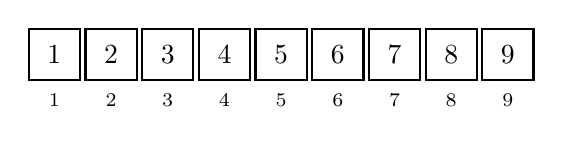
\begin{tikzpicture}
        \foreach \v [count=\i] in {1,2,3,4,5,6,7,8,9} {
            \node[draw, thick, minimum size=0.65cm, inner sep=0pt] (a\i) at (\i*0.72,0) {$\v$};
            \node[below=1pt, font=\scriptsize] at (a\i.south) {$\i$};
        }
    \end{tikzpicture}
\end{center}
Тогда соответствующее дерево (в каждой вершине --- индекс среднего элемента текущего отрезка) выглядит так:
\begin{center}
    \begin{forest}
        for tree={
            circle, draw, thick,
            minimum size=1.55em, inner sep=0pt,
            font=\small,
            s sep=1.1em,
            l sep=1.1em,
            calign=fixed edge angles,
        }
        [5
            [2
                [1]
                [3
                    [, phantom]
                    [4]
                ]
            ]
            [7
                [6]
                [8
                    [, phantom]
                    [9]
                ]
            ]
        ]
    \end{forest}
\end{center}

Заметим, что это не более чем бинарное дерево, у которого быть может не заполнен лишь последний уровень (т.е. если убрать последний слой, это будет <<идеальное>> бинарное дерево).

\Exe Покажите, что это действительно так. \textit{Указание:} покажите, что если у родителя вершины ровно один ребёнок, то у текущей вершины детей быть не может.

Тогда алгоритм бинпоиска сводится к прохождению некоторого пути от корня до искомого элемента. Совершенно, очевидно, что высота такого дерева ровно $h_0 = \lfloor \log_2 n \rfloor$ (корень на нулевой глубине).
Напоминим, что количество вершин в идеальном дереве высоты $h_0$ ровно $2^{h_0 + 1} - 1$.

\St $n = 2^{h_0} - 1 + k_0$, где $k_0$ -- количество вершин на последнем слое. Очевидно, $k_0 = n - 2^{\lfloor \log_2 n \rfloor} + 1$.
\begin{proof}

    Заметим, что если убрать вершины на $h_0$-ой глубине, то у нас точно получится идеальное бинарное дерево (все слои заполнены). В идеальном бинарном дереве высоты $h_0 - 1$ ровно $2^{h_0} - 1$ вершин, а значит, обозначив количество вершин на $h_0$-ом слое за $k_0$ получаем требуемое.

\end{proof}

Далее, в силу того, что любой элемент массива равноверноятно искомый, то аналогчино для дерева: любой узел равновероятно подходящий. 
Тогда количество итераций для поиска некоторого элемента $a$ равно длине пути от корня до соответствующего узла плюс один (ведь надо учесть первую итерацию, если мы например с первого раза нашли искомый).
Далее длину пути будем обозначать за $\eta$.
Обозначим $A_h$ как множество узлов, которые находятся на глубине $h$.
Распишем матожидание количества итераций:
\begin{equation*}
    \E \tau = \E [ \eta + 1 ] = \E \eta + 1
\end{equation*}
Далее теперь распишем матожидание длины пути, сгруппировав слагаемые. Учитываем, что длина пути от корня к вершине, есть просто глубина вершины.
\begin{equation*}
    \E \eta = \sum\limits_{h = 0}^{h_0} h \Pr[\eta = h] = \sum\limits_{h = 0}^{h_0} h \frac{|A_h|}{n} = \frac{1}{n} \sum\limits_{h = 0}^{h_0} h |A_h|
\end{equation*}
Вспомним нашу декомпозицию дерева на <<идеальную>> часть и последний слой. В каждом слое идеальной части ровно $2^h$ вершин на $h$-ом слое ($h = 0$ для корня).
А в последнем слое у нас ровно $k_0 = n - 2^{\lfloor \log_2 n \rfloor} + 1$ вершин.
\begin{multline*}
    \E \eta = \frac{1}{n} \sum\limits_{h = 0}^{h_0} h |A_h| = \frac{1}{n} \left[ \sum\limits_{h = 0}^{h_0 - 1} h |A_h| + h_0 |A_{h_0}| \right] = \\
    =  \frac{1}{n} \left[ \sum\limits_{h = 0}^{h_0 - 1} h 2^h + h_0 |A_{h_0}| \right] =  \frac{1}{n} \left[ \sum\limits_{h = 0}^{h_0 - 1} h 2^h + \lfloor \log_2 n \rfloor \left(n - 2^{\lfloor \log_2 n \rfloor} + 1\right) \right] = \EqStar{eq:binsearch-eta}
\end{multline*}

Отдельно распишем первую сумму:
\begin{multline*}
    \sum\limits_{h = 0}^{h_0 - 1} h 2^h = \sum\limits_{h = 1}^{h_0 - 1} h 2^h = \sum\limits_{h=1}^{h_0 - 1} \sum\limits_{k = h}^{h_0 - 1} 2^k = \sum\limits_{h=1}^{h_0 - 1} \left[\sum\limits_{k = 1}^{h_0 - 1} 2^k  - \sum\limits_{k = 1}^{h - 1} 2^k \right] = \\
    = (h_0 - 1) \left(2^{h_0} - 2\right) - \sum\limits_{h=1}^{h_0 - 1} \sum\limits_{k = 1}^{h - 1} 2^k = (h_0 - 1) \left(2^{h_0} - 2\right) - \sum\limits_{h=1}^{h_0 - 1} \sum\limits_{k = 1}^{h - 1} 2^k = \\
    = (h_0 - 1) \left(2^{h_0 } - 2\right) - \sum\limits_{h=1}^{h_0 - 1} \left[ 2^{h} - 2 \right] = \\
    = (h_0 - 1) \left(2^{h_0} - 2\right) + 2(h_0 - 1) - \sum\limits_{h=1}^{h_0 - 1} 2^{h} = (h_0 - 1) 2^{h_0} - 2^{h_0} + 2 = \\
    = (h_0  - 2) 2^{h_0} + 2 = \left( \lfloor \log_2 n \rfloor - 2 \right)2^{\lfloor \log_2 n \rfloor} + 2
\end{multline*}

Подставим обратно:
\begin{multline*}
    \EqStarRef{eq:binsearch-eta} = \frac{1}{n} \left[ \left( \lfloor \log_2 n \rfloor - 2 \right)2^{\lfloor \log_2 n \rfloor} + 2 + \lfloor \log_2 n \rfloor \left(n - 2^{\lfloor \log_2 n \rfloor} + 1\right) \right] = 
    \\ = \frac{1}{n} \left[ 2 - 2^{\lfloor \log_2 n \rfloor + 1} + n \lfloor \log_2 n \rfloor + \lfloor \log_2 n \rfloor \right] = \\
    = \lfloor \log_2 n \rfloor + \frac{2 - 2^{\lfloor \log_2 n \rfloor + 1} + \lfloor \log_2 n \rfloor}{n}
\end{multline*}
Итого:
\begin{equation*}
    \E \eta = \lfloor \log_2 n \rfloor + \frac{2 - 2^{\lfloor \log_2 n \rfloor + 1} + \lfloor \log_2 n \rfloor}{n}
\end{equation*}
Значит:
\begin{equation*}
    \E \tau = \lfloor \log_2 n \rfloor + 1 + \frac{2 - 2^{\lfloor \log_2 n \rfloor + 1} + \lfloor \log_2 n \rfloor}{n}
\end{equation*}

\Exe Покажите, что $\E \tau = \Theta(\log n)$.

Проверим же на практике эту оценку. Будем брать массив размера $n$ и $R$ раз запускать бинпоиск, выбирая равновероятно случайный элемент. После получения количества итераций для каждого запуска, усредняем.
\begin{figure}[H]
    \centering
    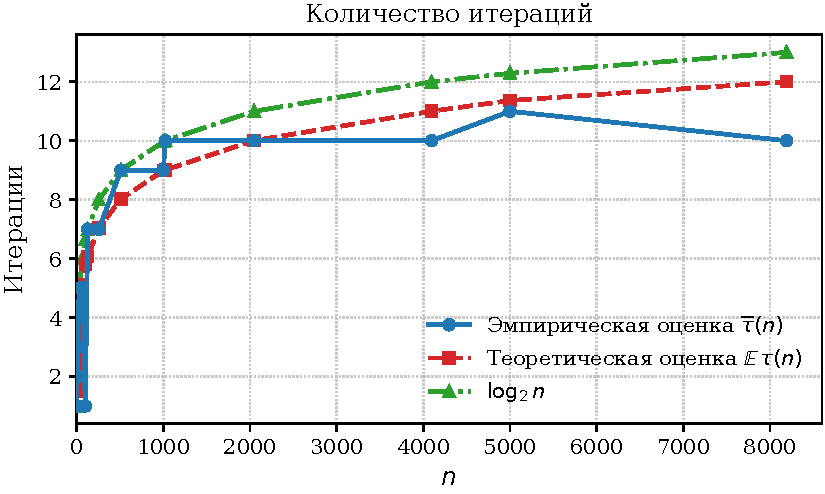
\includegraphics[width=\textwidth]{topics/probability/media/math_exp/bin_search_exp/r_1.pdf}
    \caption{$R = 1$}
\end{figure}
\begin{figure}[H]
    \centering
    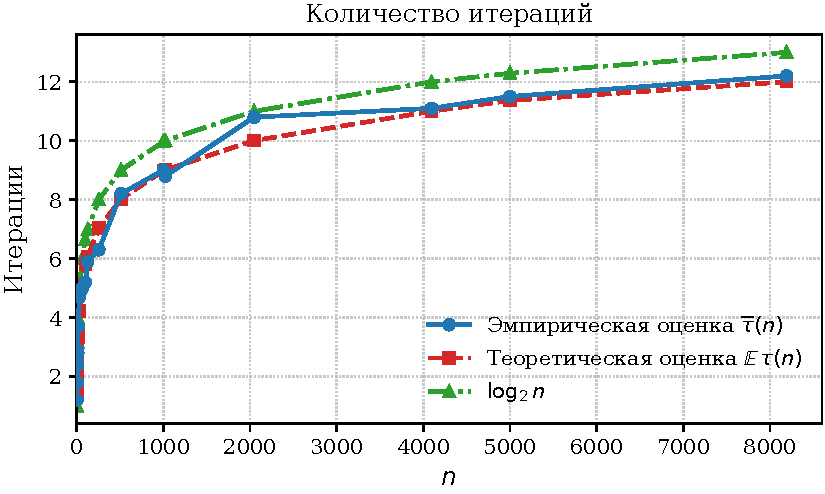
\includegraphics[width=\textwidth]{topics/probability/media/math_exp/bin_search_exp/r_10.pdf}
    \caption{$R = 10$}
\end{figure}
\begin{figure}[H]
    \centering
    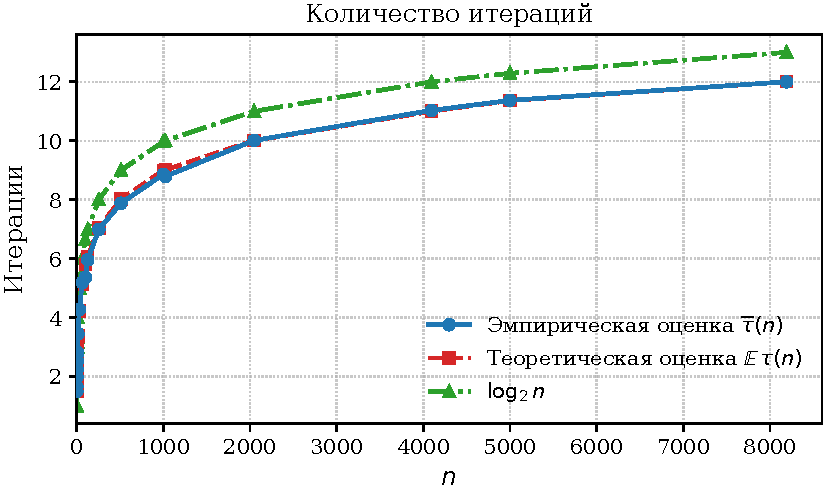
\includegraphics[width=\textwidth]{topics/probability/media/math_exp/bin_search_exp/r_100.pdf}
    \caption{$R = 100$}
\end{figure}
\begin{figure}[H]
    \centering
    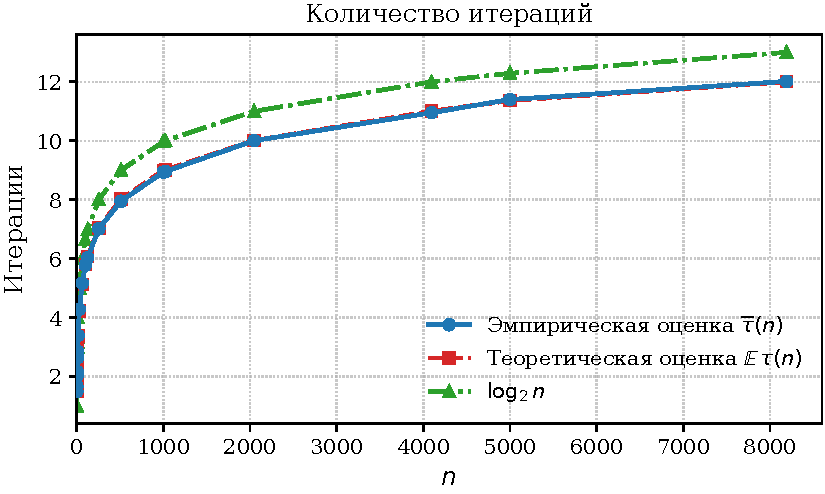
\includegraphics[width=\textwidth]{topics/probability/media/math_exp/bin_search_exp/r_1000.pdf}
    \caption{$R = 1000$}
\end{figure}

Как видим, с ростом $R$ мы все ближе и ближе приближаемся к нашей теоретической оценке среднего. Такое поведение объясняется законом больших чисел, который также остается за рамками нашего курса.
